\RequirePackage{fix-cm}
\documentclass[oneside, a4paper]{book}
\usepackage[a4paper,width=150mm,top=25mm,bottom=25mm,bindingoffset=6mm]{geometry}

% Required for inserting images
\usepackage{eso-pic,graphicx}
% misc
\usepackage{caption}
\DeclareCaptionType{equ}[][]
%\captionsetup[equ]{labelformat=empty}
\usepackage{subcaption}
\usepackage{multicol}
\usepackage{float}
\usepackage{adjustbox} % oversized table

% appendix
\usepackage[toc]{appendix}

% Default font to sans serif
\renewcommand{\familydefault}{\sfdefault}
\RequirePackage[T1]{fontenc} 
\RequirePackage[tt=false, type1=true]{libertine} 
\RequirePackage[varqu]{zi4} 
% \RequirePackage[libertine]{newtxmath}

% chapters and headers
\usepackage[Conny]{fncychap}

\usepackage{fancyhdr}
\pagestyle{fancy}
\renewcommand{\headrulewidth}{0.1pt}
\renewcommand{\chaptermark}[1]{\markboth{\MakeUppercase{\textsf{{#1}}}}{}}
\renewcommand{\sectionmark}[1]{\markright{\MakeUppercase{\textsf{\thesection\ #1}}}{} }

% section styling
\usepackage{titlesec}

% algorithms
\usepackage{algorithm}
\usepackage{algpseudocode}

% theorems and definitions
\usepackage{amsthm}
\newtheorem{definition}{Definition}

% better tables
\usepackage{tabu}

% FAT FONTS
\usepackage{bm} % bold fonts in math mode
\newcommand\fat[1]{{\boldmath{\textbf{#1}}}}
\newcommand\emphasis[1]{{\scshape\bfseries#1}}

% mathematical fonts and graphics
\usepackage{mathtools}
\usepackage{xfrac} % sfrac for diagonal slashes in fractions
\usepackage{amsfonts} % math fonts
\usepackage{amssymb} % more math symbols (supsetneq etc.)
\usepackage{dbnsymb}
\usepackage{dsfont} % math fonts
\usepackage{bbm} % mathbb fonts
\usepackage{mathrsfs} % fancy swirly font
\usepackage{gensymb} % degree sign

% draw graphs
\usepackage[inline]{asymptote}
\usepackage{qtree}
\usepackage{tikz}
\usetikzlibrary{calc}

% nicer fractions
\usepackage{xfrac}
% cancel terms
\usepackage{cancel}

% units
\usepackage{siunitx}

% plots
\usepackage{pgfplots}
\usepackage{pgfplotstable}
\usepgfplotslibrary{external}
\usepgfplotslibrary{patchplots}
\usepgfplotslibrary{groupplots}
\pgfplotsset{compat=1.18} 
\tikzexternalize[prefix=tikz,optimize=false]

% define the Spectral_r color scheme
\usepackage[table, dvipsnames]{xcolor}
\definecolor{Spectral0}{RGB}{158, 1, 66}
\definecolor{Spectral1}{RGB}{213, 62, 79}
\definecolor{Spectral2}{RGB}{244, 109, 67}
\definecolor{Spectral3}{RGB}{253, 174, 97}
\definecolor{Spectral4}{RGB}{254,224,139}
\definecolor{Spectral5}{RGB}{255,255,191}
\definecolor{Spectral6}{RGB}{230,245,152}
\definecolor{Spectral7}{RGB}{171,221,164}
\definecolor{Spectral8}{RGB}{102,204,204}
\definecolor{Spectral9}{RGB}{50,136,189}
\definecolor{Spectral10}{RGB}{94,79,162}
\pgfplotsset{
  colormap={Spectral_r}{
    rgb255(0cm)=(94,79,162)         % 0.0
    rgb255(1cm)=(50,136,189)        % 0.1
    rgb255(2cm)=(102,204,204)       % 0.2
    rgb255(3cm)=(171,221,164)       % 0.3
    rgb255(4cm)=(230,245,152)       % 0.4
    rgb255(5cm)=(255,255,191)       % 0.5
    rgb255(6cm)=(254,224,139)       % 0.6
    rgb255(7cm)=(253,174,97)        % 0.7
    rgb255(8cm)=(244,109,67)        % 0.8
    rgb255(9cm)=(213,62,79)         % 0.9
    rgb255(10cm)=(158,1,66)         % 1.0
    }
}


% get width of given text
\usepackage{calc}

% define a horizontal spacer
\newcommand\horizontalspacer[0]{\vspace{5pt}\noindent\textcolor{lightgray}{\rule{\textwidth}{1mm}}
\vspace{5pt}}

% clickable links
\usepackage{hyperref}
\hypersetup{
    colorlinks,
    citecolor=black,
    filecolor=black,
    linkcolor=black,
    urlcolor=black
}
\renewcommand{\itemautorefname}{Item}
% fancy boxes
\usepackage{fancybox}
\newcommand{\equationnamed}[2]{%
  \setlength{\fboxsep}{2pt} % padding inside box
  \setlength{\fboxrule}{0.01pt}
  \begin{center}
    \begin{minipage}{\textwidth}
      \begin{center}\textsc{#1}\end{center}
      #2
    \end{minipage}
  \end{center}
}
\newcommand{\equationnamedbox}[2]{%
  \setlength{\fboxsep}{5pt} % padding inside box
  \setlength{\fboxrule}{0.01pt}
  \begin{center}
    \fbox{
      \begin{minipage}{0.4\textwidth}
        \begin{center}\emphasis{#1}\end{center}
        #2
      \end{minipage}
    }
  \end{center}
}

% labels to enum items
\usepackage{enumitem}

\usepackage{array}

% make empty lines skip
% \usepackage{parskip}

% include pdfs 
\usepackage{pdfpages}

% code
\usepackage{minted}
\usepackage{listings}

% ~~~~~~~~~ TYPESETTING AND OTHER MACROS ~~~~~~~~~~~~~~~~~~~~~

\newenvironment{absolutelynopagebreak}
  {\par\nobreak\vfil\penalty0\vfilneg
   \vtop\bgroup}
  {\par\xdef\tpd{\the\prevdepth}\egroup
   \prevdepth=\tpd}

% ~~~~~~~~~ AFANCY CHAPTER HEADINGS ~~~~~~~~~~~~~~~~~~~~~~~~~~~
\makeatletter
\def\thickhrulefill{\leavevmode \leaders \hrule height 1ex \hfill \kern \z@}
\def\@makechapterhead#1{%
  %\vspace*{50\p@}%
  \vspace*{10\p@}%
  {\parindent \z@ \centering \reset@font
        \thickhrulefill\quad
        \scshape \@chapapp{} \thechapter
        \quad \thickhrulefill
        \par\nobreak
        \vspace*{10\p@}%
        \interlinepenalty\@M
        \hrule
        \vspace*{10\p@}%
        \Huge {\textbf{#1}} \par\nobreak
        \par
        \vspace*{10\p@}%
        \hrule
    \vskip 40\p@
    % \vskip 100\p@
  }}
\def\@makeschapterhead#1{%
  %\vspace*{50\p@}%
  \vspace*{10\p@}%
  {\parindent \z@ \centering \reset@font
        \thickhrulefill
        \par\nobreak
        \vspace*{10\p@}%
        \interlinepenalty\@M
        \hrule
        \vspace*{10\p@}%
        \Huge \bfseries #1\par\nobreak
        \par
        \vspace*{10\p@}%
        \hrule
    \vskip 40\p@
    % \vskip 100\p@
  }}

  \newcommand*{\@rowstyle}{}
  \newcommand*{\rowstyle}[1]{% sets the style of the next row
    \gdef\@rowstyle{#1}%
    \@rowstyle\ignorespaces%
  }
  \newcolumntype{=}{% resets the row style
    >{\gdef\@rowstyle{}}%
  }
  \newcolumntype{+}{% adds the current row style to the next column
    >{\@rowstyle}%
  }
  
\usepackage[pdftex,outline]{contour}

% ~~~~~~~~~ MATH MACROS ~~~~~~~~~~~~~~~~~~~~~~~~~~~~~~~~~~~~~~

% abs value macro
% \DeclarePairedDelimiter\abs{\lvert}{\rvert}
\newcommand\abs[1]{\left|#1\right|}
\newcommand\abss[1]{\left|\left|#1\right|\right|}
\newcommand\norm[1]{\left\lVert#1\right\rVert}
\newcommand\angled[1]{\left\langle#1\right\rangle}
\newcommand\round[1]{\left\lfloor#1\right\rceil}

\newcommand\dist[1]{\left|\left|#1\right|\right|}
\newcommand\arr[1]{\left\langle#1\right\rangle}
\newcommand\pdpi[0]{\frac{\partial}{\partial p_i}}

% define the laplace operator 
\newcommand*\Laplace{\mathop{}\!\mathbin\nabla^2}
\newcommand\vek[1]{\vec{\bm{#1}}}
\newcommand\nvek[1]{\hat{\vec{\bm{#1}}}}
\newcommand\mat[1]{{\mathds{#1}}}
\newcommand\br[1]{\left(#1\right)}

\DeclareMathOperator{\sgn}{sgn}
\DeclareMathOperator{\erf}{erf}

\DeclareMathOperator*{\argmax}{\arg\!\max}
\DeclareMathOperator*{\argmin}{\arg\!\min}

\newcommand\divergence{{\nabla\cdot}}


\author{Julian Karrer}
\title{Exercise 2: Convexity, Duality and Fitting problems}

\begin{document}
\chapter{Root finding of a convex 1D function}
Let $f: \mathds{R}\to\mathds{R}$ be differentiable, strictly monotonously increasing and convex with some $x^*$ such that $f(x^*)=0$
\begin{itemize}
    \item Since the function is strictly monotonous it has at most one root, so $x^*$ is the unique root 
    \item If $x_k \geq x^*$ then also $x_{k+1}\geq x^*$ due to convexity, since tangents lie below the graph, and since the gradient is positive due to strict monotonocity
    \item Suppose $x_0 < x^*$, then due to convexity the tangent at $x_0$ is below the graph and $x_1\geq x^*$
    \item So after at most one iterate $x^* \leq x_k$ is a lower bound of the sequence of all $x_k$s
    \item Further, $x_{k+1} = x_k - \frac{f(x_k)}{f'(x_k)}$ where $f(x_k)\geq 0$ since $x_k$ is greater than the root of a strictly monotonous function and $f'(x_k)>0$ due to strict monotonicity
    \item Therefore $\frac{f(x_k)}{f'(x_k)} > 0$ and $x_{k+1} < x_k$, so the sequence of $x_k$ strictly monotonously decreases
    \item Since the sequence of $x_k$ strictly monotonously decreases and is lower-bound by $x^*$, it converges to $x^*$ $\qed$
\end{itemize}


\chapter{Regularization}
\[
  \mathrm{Z\kern-.3em\raise-0.5ex\hbox{Z}}: 
  \lim_{\lambda\to\infty} \br{x_k - \br{B_k - \mathds{I}}^{-1} \nabla f(x_k) }= x_k - \frac{1}{\lambda}\nabla f(x_k) + \mathcal{O}\br{\frac{1}{\lambda^2}}
\]
\begin{align*}
  x_{k+1} &= x_k - \br{B_k + \lambda \mathds{\mathds{I}}}^{-1} \nabla f(x_k)\\
  &= x_k - \br{\lambda \frac{1}{\lambda} B_k + \lambda \mathds{I}}^{-1} \nabla f(x_k)\\
  &= x_k - \frac{1}{\lambda}\br{\frac{1}{\lambda} B_k + \mathds{I}}^{-1} \nabla f(x_k)\\
  &= x_k - \frac{1}{\lambda}\br{\mathds{I} -\underbrace{\br{-\frac{1}{\lambda} B_k}}_{=: B'}}^{-1} \nabla f(x_k)\\
\end{align*}
Since $\rho(B') \propto \frac{1}{\lambda}$ there exists some $\lambda_0$ such that $\forall \lambda>\lambda_0: \rho(B')<1$ and the geometric series expansion is applicable to the limit $\lambda \to \infty$
\begin{align*}
  x_{k+1} &=  x_k - \frac{1}{\lambda}\br{\mathds{I} + B' + B'^2 + \dots} \nabla f(x_k)\\
  &=  x_k - \frac{1}{\lambda} \nabla f(x_k) \underbrace{
    + \frac{1}{\lambda^2} B_k^2 \nabla f(x_k) 
    - \frac{1}{\lambda^3} B_k^3 \nabla f(x_k) 
    + \dots
    }_{\in\mathcal{O}\br{ \frac{1}{\lambda ^2} }}\\
  &=  x_k - \frac{1}{\lambda} \nabla f(x_k) + O\br{\frac{1}{\lambda^2}}\qed\\
\end{align*}

\chapter{Unconstrained minimization}
\begin{enumerate}
  \item \begin{align*}
    f(x,y) &= \frac{1}{2}(x-1)^2 + \frac{1}{2}y^2+\rho\frac{1}{2}(y-\cos(x))^2\\
    \frac{\partial}{\partial x} f(x,y) &= x - 1 + \rho\sin(x)(y-\cos(x))\\
    &= x + \rho y\sin(x)-\frac{\rho}{2}\sin(2x) - 1 \\
    \frac{\partial}{\partial y} f(x,y) &= y (1 + \rho) -\rho \cos(x)\\
    \Longrightarrow \nabla f &= \begin{bmatrix}
      x + \rho y\sin(x)-\frac{\rho}{2}\sin(2x) - 1\\
      (1 + \rho)y  -\rho \cos(x)
    \end{bmatrix}\\
    \frac{\partial^2}{\partial x^2}f &= 1 + \rho y \cos(x) -\rho\cos(2x)\\
    \frac{\partial^2}{\partial y^2}f &= 1 + \rho\\
    \frac{\partial}{\partial y}\br{\frac{\partial}{\partial x}f} &=  \rho\sin(x) =  \frac{\partial}{\partial x}\br{\frac{\partial}{\partial y}f}\\
    \Longrightarrow \nabla^2 f &= \begin{bmatrix}
      1 + \rho y \cos(x) -\rho\cos(2x) & \rho\sin(x) \\
      \rho\sin(x) &  1 + \rho
    \end{bmatrix}
  \end{align*}
  \item \begin{align*}
    f(x,y) &= \frac{1}{2}(x-1)^2 + \frac{1}{2}y^2+\rho\frac{1}{2}(y-\cos(x))^2\\
    &= \frac{1}{2}\br{(x-1)^2 + y^2 + \rho(y-\cos(x))^2}\\
    &=  \frac{1}{2} \abss{\begin{bmatrix}
      (x-1)\\
      y\\
      \sqrt{\rho}\br{y-\cos(x)}
    \end{bmatrix}}^2\\
    &=: \frac{1}{2}\abss{r(x,y)}^2
  \end{align*}
  \item \begin{align*}
    J_r &= \begin{bmatrix}
      1 & 0\\
      0 & 1\\
      \sqrt{\rho}\sin(x) & \sqrt{\rho}
    \end{bmatrix}\\
    B_k &= J_r^T J_r\\
    &= \begin{bmatrix}
      1 & 0 & \sqrt{\rho}\sin(x)\\
      0 & 1 & \sqrt{\rho}
    \end{bmatrix}\begin{bmatrix}
      1 & 0\\
      0 & 1\\
      \sqrt{\rho}\sin(x) & \sqrt{\rho}
    \end{bmatrix}\\
    &= \begin{bmatrix}
      1 + \rho\sin^2(x) & \rho\sin(x)\\
      \rho\sin(x) & 1 + \rho
    \end{bmatrix}
  \end{align*}
  \item The approximate Hessian is therefore equal to the exact Hessian when:
  \begin{align*}
    1 + \rho y \cos(x) -\rho\cos(2x) &= 1 + \rho\sin^2(x) & | -1 \quad|\cdot\frac{1}{\rho}\\
    y \cos(x) -\cos(2x) &= \sin^2(x) & |\cos(2x)=1-2\sin^2(x)\\
    y \cos(x) + 2\sin^2(x) -1 &= \sin^2(x) & |-\sin^2(x)\\
    y \cos(x) + \sin^2(x) &= 1 &\\
  \end{align*}
  \item see \autoref{fig:3d} and \autoref{fig:value}
  \item All methods appear to converge to the same minimum. The Gauss-Newton converges fastest in this instance, followed by the exact Newton's method. Gradient descent makes rapid progress comparable to Gauss-newton at the beginning, but tapers off as it slowly progresses along a relatively flat ridge in the function landscape.
\end{enumerate}

\begin{figure}[H]
    \centering
    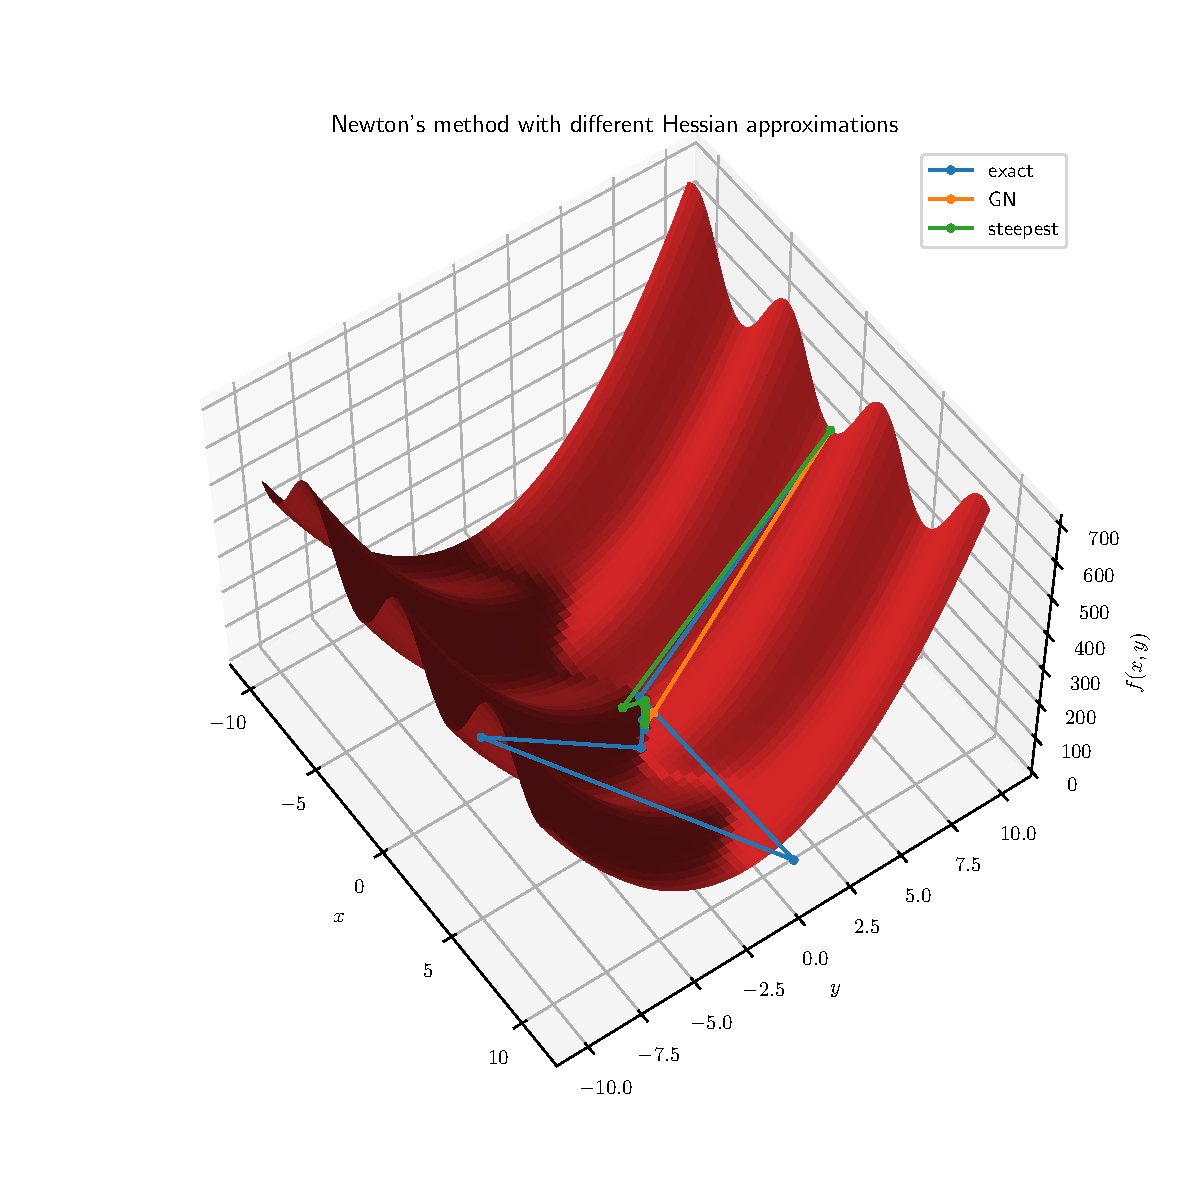
\includegraphics[width=\linewidth]{3d.pdf}
    \caption{3D surface visualization of the descent using different Hessian approximations}
    \label{fig:3d}
\end{figure}

\begin{figure}[H]
  \centering
  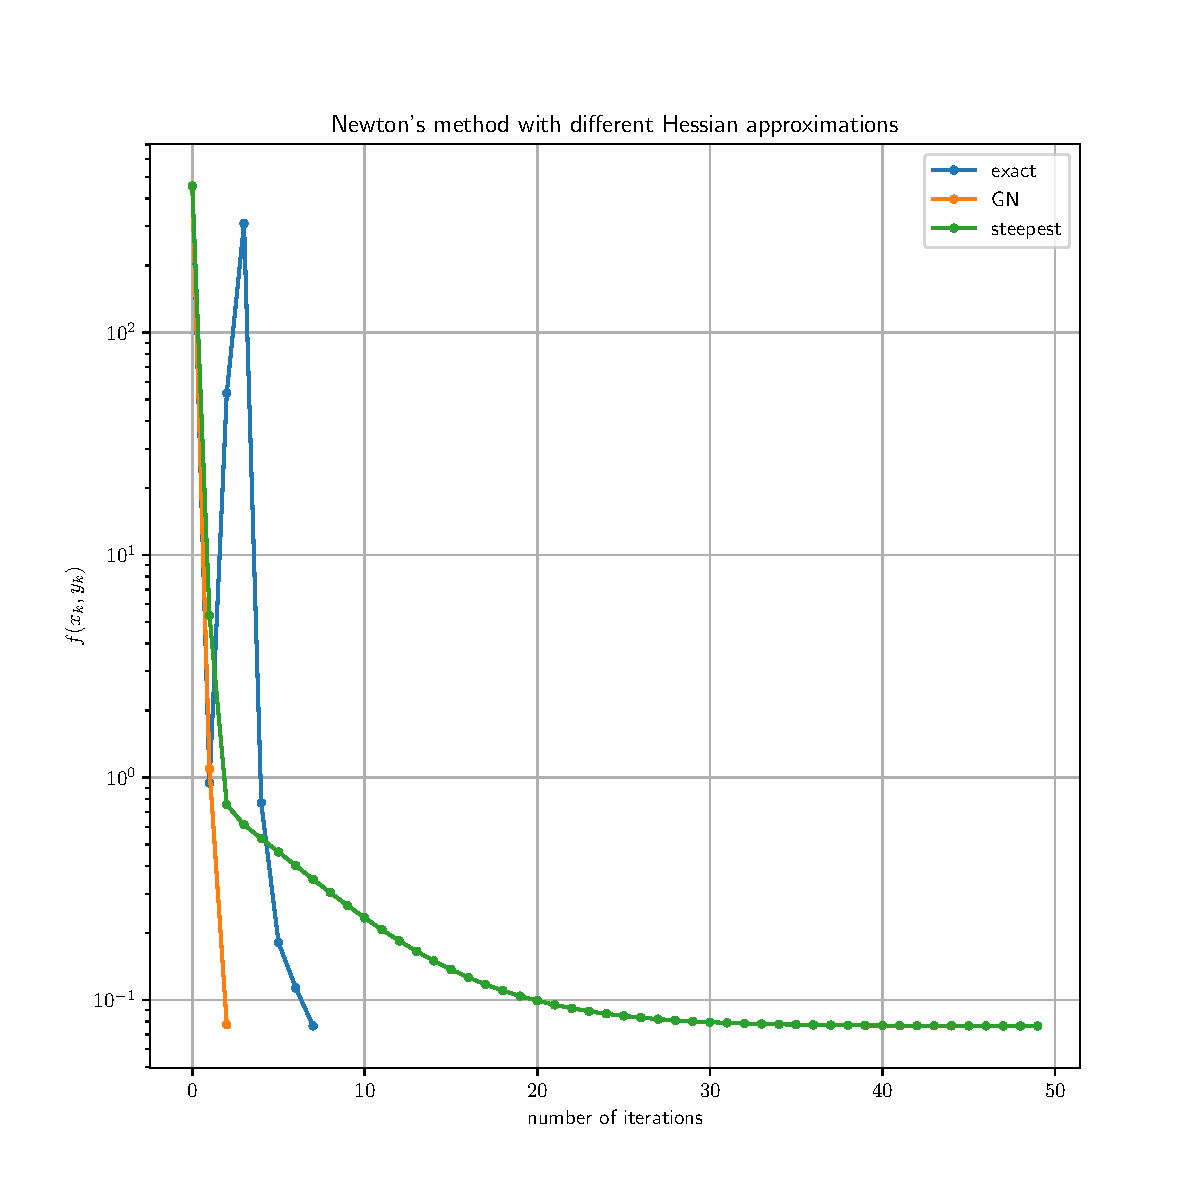
\includegraphics[width=\linewidth]{value.pdf}
  \caption{Function values per iteration of the different Hessian approximations}
  \label{fig:value}
\end{figure}

\chapter{Hanging chain, revisited}
\begin{figure}[H]
  \centering 
  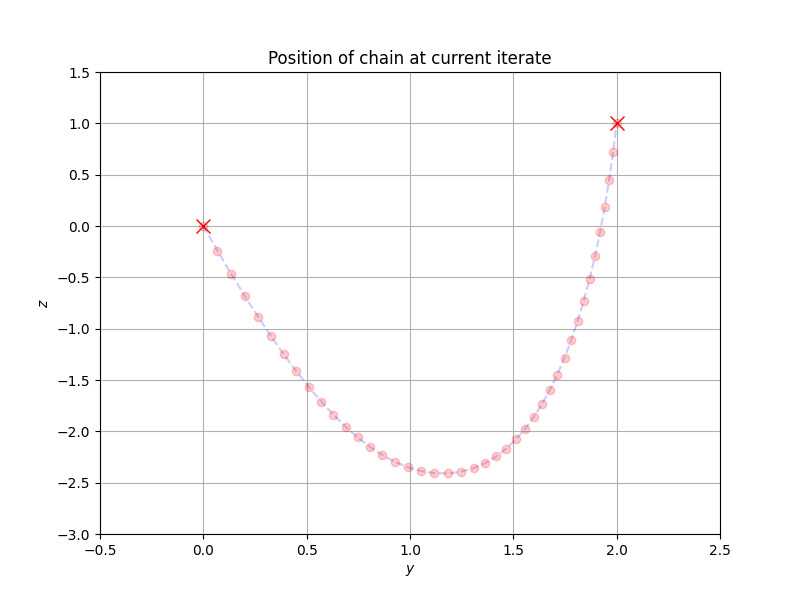
\includegraphics[width=\textwidth]{screenshot.png}
  \caption{The algorithm converges to the expected solution}
  \label{fig:hanging-chain}
\end{figure}

\chapter{Source Code}

\section{Unconstrained Newton-Type Methods}
\inputminted{python}{unconstrained_newton.py}
\section{Hanging Chain}
\inputminted{python}{hanging_chain_next_episode.py}


\end{document}